\section{Modelo de Arquitetura} 
O modelo do nosso projeto(demonstrado na figura 3) é constituído por três módulos principais: uma REST API, e duas aplicações cliente: uma orientada à plataforma \textit{mobile} Android e outra desenvolvida para ser usada num \textit{browser}.
\par \medskip

	A API estabelecerá endpoints onde será possível executar pedidos HTTPS de maneira a suportar autenticação e operações na infraestrutura (criação de perfil, “seguimento” de organização, inscrição em ação de voluntariado, etc.). Esta API representa o \textit{back-end} do projeto.
\par \medskip

Serão então implementadas duas aplicações cliente, constituindo o \textit{front-end}: 
\begin{itemize}
	\item um cliente \textit{mobile}, para a plataforma Android, usado pelos voluntários. Nesta interface será possível efetuar por parte do utilizador as operações de uso da plataforma usuais: criação de um perfil, visionamento de um \textit{feed} de \textit{posts} efetuados pelas organizações seguidas, entre outras;
	\item um cliente \textit{browser}. Esta aplicação é direcionada às organizações e terá a finalidade de permitir às mesmas realizar \textit{posts}, criar e gerir ações de voluntariado, etc.;
\end{itemize}

\begin{figure}[h]
	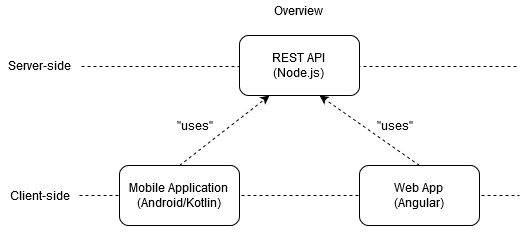
\includegraphics[scale=.8]{architecture}
	\caption{Modelo de arquitetura}
\end{figure}

\subsection{REST API}
(todo)

\subsection{\textit{Mobile App}}
(todo)

\subsection{\textit{Web App}}
(todo)

\subsection{Tecnologias e ferramentas}
(todo)